\chapter{REFERÊNCIA TEÓRICA}

O presente capítulo tem por objetivo a contextualização, de forma generalizada, a análise de sentimentos, cobrindo a sua origem, suas principais aplicações nas mais diversas áreas do conhecimento, com especial à economia, como também os trabalhos preponderantes que inspiram essa pesquisa. Além disso, será feita uma breve análise sobre os mercados e contexto econômico desta monografia.

\section{Análise de Sentimentos}

O avanço tecnológico nos permitiu invenções dignas de histórias de ficção científica, sendo a principal delas a Internet, que hoje nos permite acessar qualquer informação na palma de nossas mãos em segundos e assim democratizar o conhecimento mundialmente. Com ela, vimos que não só obtemos conhecimento quase que ilimitado, mas como geramos informações em proporções nunca antes vistas. Estima-se que geramos 2,5 quintilhões de bytes de dados todos os dias \citeonline{ibm}, informação superior em milhares de vezes às que geramos nos últimos dois milênios de história humana.

Disso se cunhou no início do século 21 o termo \textit{Big Data}, o qual se refere a toda grande gama de dados que são criados e que são usados para obter, armazenar, tratar e analisar esses dados. O estudo da \textit{Big Data} compreende também o uso dessa informação para prever (ou ao menos tentar) acontecimentos futuros a partir dos dados passados e como isso pode favorecer a sociedade em geral. A Figura \ref{fig: bigdata} ilustra a popularização do termo através dos anos, chegando ao seu auge nos anos recentes.  

\begin{figure}[!h]
    \centering
    \caption{Evolução de buscas pelo termo Big Data - de 2004 à 2022}
    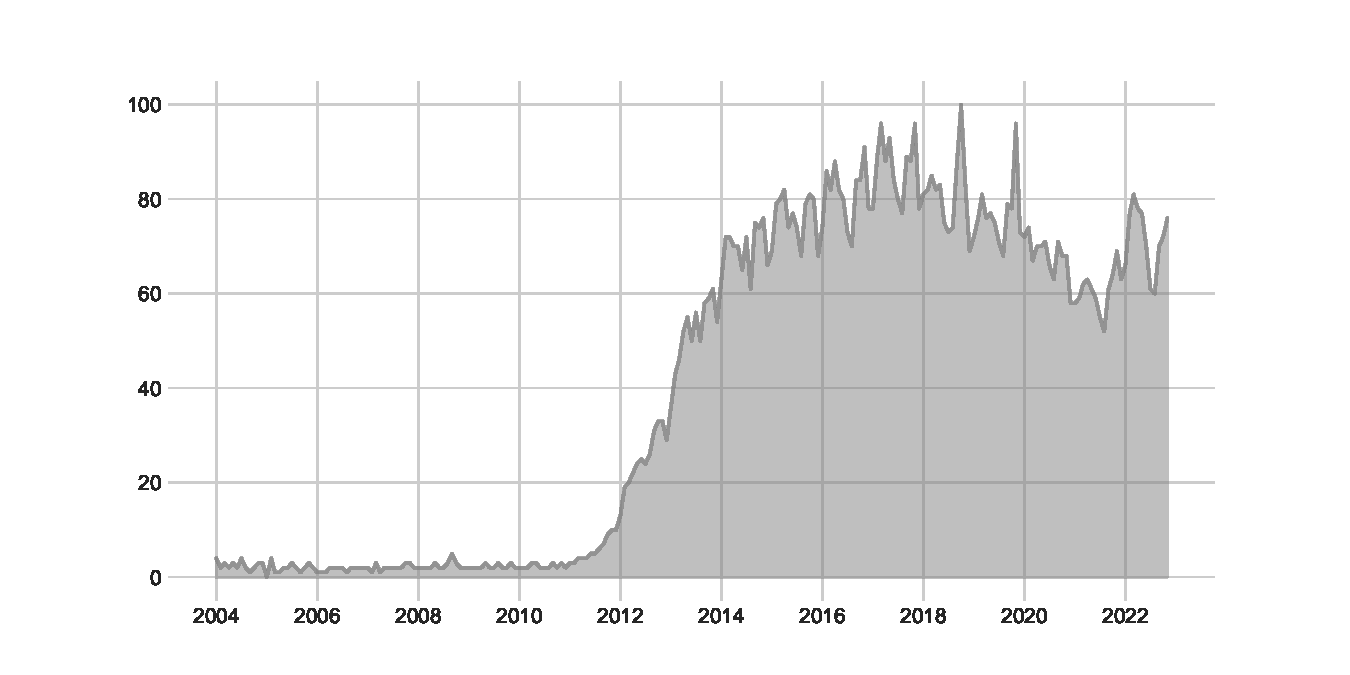
\includegraphics[width=0.9\textwidth]{imagens/bigdata_google.pdf}
    \label{fig: bigdata}
    \caption*{Fonte: Google Trends. Elaboração Própria}
\end{figure}

Diante dessa revolução tecnológica, perguntas e questionamentos são levantados de como essa imensa quantidade de dados pode contribuir para a melhoria do bem-estar da população sem violar os seus direitos e privacidade \citeonline{datahealth}. E, em como qualquer revolução, a sociedade se defronta com novos desafios e oportunidades a serem discutidas e exploradas.

A partir dos avanços alcançados pela tecnologia e tão recentes estudos da \textit{Big Data} possibilitaram também a criação de novas formas de análise e processamento de textos, como as técnicas de mineração textual e análise de sentimentos, haja visto a tremenda quantidade de conteúdo escrito que é despejado nas redes por segundo. Essas técnicas surgiram através da ciência da computação e linguística pelo subcampo da \textit{Natural Language Processing} que estuda os fenômenos linguísticos nos conteúdos escritos. A NLP é normalmente empregada em aplicações que envolvam Inteligência Artificial (IA), na expectativa de treinar e ensinar computadores a aprenderem de forma natural e produzirem por si próprios conteúdos escritos. Diferentemente do \textit{text mining} e \textit{sentiment analysis} que são técnicas empregadas para extrair (\textit{mining}) e analisar suas informações com o foco em identificar sentimentos e emoções em textos. 

Ferramentas como estas são comuns nas últimas décadas, sendo realizados métodos semelhantes nos campos dos negócios, marketing, ciências sociais, política, dentre outros. Entretanto, por mais que sejam semelhantes em teoria, a prática das duas se diferem em técnica, sendo mais comum a busca de termos mais frequentes, a forma que o conteúdo é redigido, a busca de termos específicos, entre outros. Enquanto que a mineração de textos se ocupa com textos não estruturados que em essência não possuem forma e conteúdo bem definidos, como os textos advindos de redes sociais, blogs, sites, dentre qualquer outro meio escrito vinculada à \textit{world wide web}. E, a análise de sentimentos, que se preocupa em desvendar os sentimentos e emoções exprimidos em qualquer tipo textual, sejam elas positivas ou negativas. Além disso, também servem para mensurar o nível de otimismo ou pessimismo de um texto, a sua polarização e avaliar sentenças e opiniões.

\begin{figure}[!h]
    \centering
    \caption{Evolução de buscas pelo termo Análise de Sentimentos - de 2004 à 2022}
    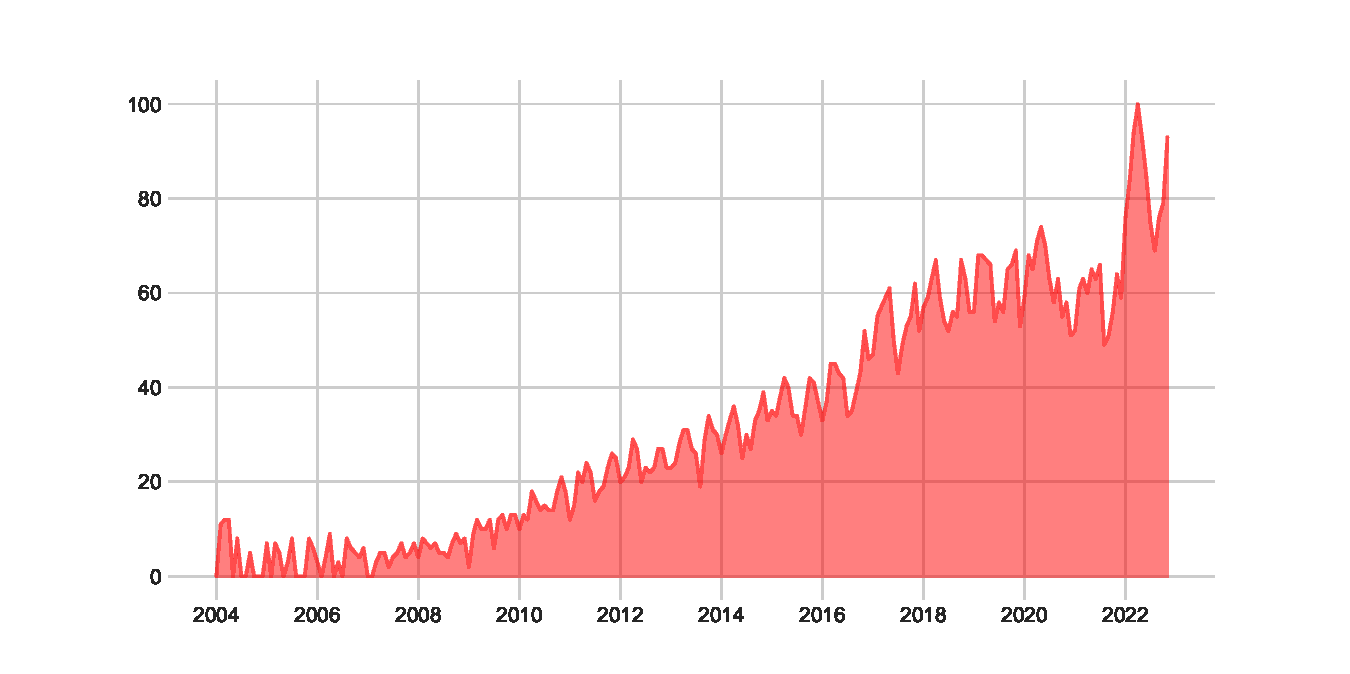
\includegraphics[width=0.8\textwidth]{imagens/sentimentanalysis_google.pdf}
    \label{fig: sentiment}
    \caption*{Fonte: Google Trends. Elaboração Própria}
\end{figure}

Em resumo, a análise de sentimentos busca extrair sentimentos e emoções de conteúdos escritos e devido ao grande avanço tecnológico, a sua aplicação tem crescido nos diversos campos do conhecimento. Tal crescimento pode ser enxergado na Figura \ref{fig: sentiment}, demonstrando o aumento ano-a-ano de buscas pelo assunto. 

Dentro disso, existem duas formas comuns para classificação de texto: categórica ou grandeza. Na forma categórica, o texto em questão adquire valores categóricos entre positivo, negativo ou neutro. Na técnica de grandeza, o termo recebe uma classificação escalar com valores entre 1 à 5 ou -1 à 1, a depender do método utilizado \cite{shap-sud}.

Vale aqui mencionar os diferentes métodos computacionais para a análise de sentimentos, sendo os mais comuns a abordagem pela \textit{lexicon methodology} e a de \textit{machine learning techniques}. O primeiro método utiliza listas pré-definidas de palavras ou sentenças, chamadas de \textit{lexicons} ou \textit{dictionaries}, onde cada palavra assume uma nota (\textit{score}) para a emoção de interesse. Enquanto o segundo, emprega técnicas de ML para a construção de modelos complexos que possibilitem a previsão dos sentimentos num conjunto de texto. Ou seja, os modelos que utilizam ML procuram aprender com textos pré-definidos contendo mapeamento entre declarações textuais e classificações de sentimentos assumidas por humanos. 

Diante da gama de métodos e modelos existentes, é importante salientar que a literatura de \textit{sentiment analysis} enfatiza pontos focais para a caracterização de sentimentos: seu domínio e complexidade. O domínio é crucial, pois idealmente a análise de sentimentos deve apropriar-se do domínio do texto que a ferramenta está sendo aplicada. 

Em suma, na análise de sentimentos, para se obter resultados mais acurados e não-viesados, é necessário que o modelo usado no estudo contenham termos apropriados ao domínio ao qual está sendo treinado.

\subsection{VADER}

O algoritmo VADER (\textit{Valence Aware Dictionary for Sentiment Reasoning}) é um modelo computacional para análise de sentimentos desenvolvido por \citeonline{vader}, expoentes da ciência da computação. Esse modelo surge em resposta às grandes dificuldades inerentes à aplicabilidade de análise de sentimentos em mídias sociais.

Seus autores criam um dicionário baseado na valência da sentença, dessa forma, seu método parte de, para cada termo contido no corpus, lhe é atribuído um valor específico em ordem de obter a sua intensidade. Isto é, para cada termo contido no corpus de texto é dado um valor de grandeza escalar para representar a intensidade de seu sentimento, seja positivo ou negativo.

Utilizando uma gama de métodos qualitativos e quantitativos, os autores constroem e testam empiricamente uma lista de palavras, \textit{lexicon}, adaptadas ao contexto de microblogs e redes sociais para validação do seu modelo. 

Dessa forma, o dicionário VADER apresenta um método alternativo para análise de sentimento, empregando um formato de grandeza para classificação de sentimentos por meio de um modelo de regras simples.

Para compreensão da efetividade do modelo, os autores \citeonline{vader} comparam-o com as principais ferramentas disponíveis no mercado para análise de sentimentos e também com técnicas desenvolvidas a partir do aprendizado de máquina. Seus resultados demonstraram que seu modelo era mais efetivo que todos os \textit{benchmarks}. Além disso, pode ser percebido que seu modelo performou melhor do que as classificações individuais feitas por seres humanos.

Em suma, o dicionário VADER demonstra ser um grande artifício para análise de sentimentos, comprovando ser mais efetivo do que as principais ferramentas para compreensão de sentimentos disponíveis atualmente. Entretanto, apesar de ser um dicionário para toda gama de textos, seus resultados demonstram ser melhor quando aplicados ao contexto de redes sociais, campo no qual foi idealizado. Por esse motivo, suas aplicações se limitam a esse meio, sendo vistos uma queda de performance quando aplicados a outros contextos. 

O algoritmo VADER pode ser encontrado no pacote \textit{nltk}, proposto por \citeonline{nltk}, construído para criação e aplicação de algoritmos e programas para processamento de linguagem natural.


\section{Análise de Sentimentos e Economia}

O uso destes métodos tem se popularizado bastante há alguns anos, principalmente pelo aumento da velocidade de processamento de dados, geração de informações inimagináveis e novos meios pelos quais essas técnicas podem ser empregadas. Porém, seu uso no campo econômico tem sido recente, tendo em vista às novas vantagens teóricas e empíricas que ela pode ser aplicada. 

Trabalhos acadêmicos recentes têm começado a explorar esse campo do conhecimento, com aplicações que vão desde a criação de índices econômicos para avaliar a confiança do consumidor através das notícias até a avaliação de retornos de investimentos pelo nível de positividade e negatividade em artigos econômicos, tornando assim muito amplo as aplicações que a análise de sentimentos possui. Citarei alguns exemplos de aplicações a seguir.

\subsection{Medição de sentimentos em notícias (Measuring News Sentiment)}

Em \textit{Measuring News Sentiment}, os autores \citeonline{shap-sud} incorporam técnicas de \textit{text sentiment analysis} para desenvolver uma medida de série temporal que demonstre o nível de confiança (humor) expresso nas notícias econômicas e financeiras. Portanto, é construído um índice de sentimentos a partir das notícias econômicas a fim de medir o nível de incerteza ou otimismo da economia. Para isto, foram selecionados milhares de artigos econômicos e financeiros dos Estados Unidos e comparados com dados econômicos do país.

Os autores partem do princípio de que \textit{policymakers} e agentes do mercado tomam suas decisões a partir de um amontoado de informações, sejam \textit{hard} ou \textit{soft information}. Entretanto, ao contrário das \textit{hard information} que podem ser quantificadas, como desemprego e produção, as \textit{soft information} são compostas de informações mais subjetivas. Pela sua natureza subjetiva, se tornam mais difíceis de mensurar e avaliar no campo econômico. A partir disso, modelos que agreguem outros tipos de informações são vagos dentro do meio. Por isso, os autores estudam a influência das \textit{soft information} nos fenômenos econômicos. 

Para efeito de comparação, os autores constroem o índice e os comparam com medidas de sentimento de confiança do consumidor no mercado americano, sendo eles o \textit{Index of Consumer Sentiment} da \citeonline{index-michigan} e \textit{The Consumer Confidence Survey} medida pela organização \citeonline{conferenceboard}. Essas medidas são semelhantes aos Índices de Confiança medidas pela \citeonline{indicefgv} em território brasileiro.

Pelos resultados dos autores, o \textit{news sentiment index} demonstrou forte correlação com os índices Michigan e Conference Board. O fato de que o índice dos autores se move junto aos índices de confiança demonstra que eles refletem fenômenos econômicos e não apenas ruídos.

Em seguida, os autores buscam avaliar o poder preditivo que o índice possui sobre a atividade econômica futura. Para realização deste experimento, \citeonline{shap-sud} procuram avaliar os efeitos ocorridos na economia provocados por um, "choque" no \textit{news sentiment measure}. Para o teste, decidem provocar um choque no índice de sentimentos pela Função de Resposta ao Impulso e observar o comportamento nas séries para Consumo, Produção, \textit{Real Estate} e inflação.

O teste mostrou que o choque eleva o consumo, produção e taxa de juros real, enquanto reduz levemente o nível de preços. Além disso, o efeito sob os preços é transitório, mas no restante os efeitos são mais duradouros. A similaridade dos resultados provém da alta evidência de que \textit{news sentiment measure} tem impacto similar aos do \textit{consumer confidence index}.

Por fim, \citeonline{shap-sud} concluem que medidas baseadas em sentimentos dos textos performam bem ao capturar informação econômica significativa. Além de terem baixo custo para implementação e utilização, os autores preveem que os avanços tecnológicos e de processamento levarão ao maior uso desse tipo de medida para avaliação econômica, tendo em vista que é esperado uma melhora nos métodos de análise textual.

\subsection{Sentimetos durante Recessões (Sentiment during recessions)}

Neste artigo, \citeonline{garcia} estuda os efeitos que os sentimentos dos jornais possuem nos preços dos ativos durante o século XX (1905-2005). A \textit{proxy} para sentimento é criada a partir da fração de termos positivos e negativos contidos em duas colunas do jornal \citeonline{nytimes}.

Como citado pelo autor, \citeonline{shiller} argumenta que notícias de mídia são um importante componente para acompanhar movimentos de mercados e também provocá-los. Partindo desse pressuposto, \citeonline{garcia} formula seu argumento de que investidores seguem manchetes como fonte informacional para tomarem suas decisões, sugerindo que o sentimento do mercado é refletido por conteúdos de notícias e mídia em geral.

Além disso, a literatura econômica e psicológica sugere que investidores são mais sensíveis às notícias durante períodos difíceis. Isto é, evidências encontradas na psicologia e da economia comportamental fomentam esta ideia, visto que em períodos de incerteza e de perdas, tomadores de decisão podem mudar seu modo de decisão, em comparação aos períodos de expansão econômica. Partindo desse ponto, o autor assume que períodos de recessão econômica correspondem com tempos de alta sensibilidade às notícias de mercado, tendo em vista que tais períodos tornam a população mais pessimista e negativa quanto ao futuro.

Para sua \textit{proxy} de sentimentos é construída a partir da contagem de palavras positivas e negativas contidas nas colunas publicadas diariamente pelo \citeonline{nytimes} que cobrem tópicos gerais de finanças, desde performance das ações à eventos macroeconômicos.

Ao comparar a fração de palavras positivas e negativas nos textos e os retornos do \textit{Dow Jones Industrial Average}, o autor encontra significância para previsão dos retornos. A fração de positividade ajuda a prever os retornos das ações, enquanto que a fração de negatividade demonstra ser significante ao prever o baixo retorno das ações. Entretanto, os efeitos das medidas de retorno das ações durante os períodos de expansão são menores do que os encontrados nos períodos de recessão, indicando que a \textit{proxy} de sentimentos tem pouco efeito sobre a primeira do que a segunda.

Por fim, o autor defende que dicionários de \textit{positive words} são tão importantes quanto as de \textit{negative words} haja vista a sua significância para identificar a previsibilidade das ações. Ademais, a maior descoberta de \citeonline{garcia} é que conteúdos de notícias contribuem na previsão de retornos das ações em sua frequência diária, sendo mais significativo durante recessões econômicas.

Em suma, considerando-se os resultados encontrados, seu artigo argumenta que o sentimento dos investidores são mais voláteis durante tempos difíceis, suportando assim as hipóteses encontradas na literatura econômica.

\subsection{Mineração de dados e Extração de Sentimentos em Documentos do Banco Central}

Em \citeonline{bruno}, o autor aplica as metodologias de mineração de texto e análise de sentimentos aos relatórios do Banco da Itália entre 1996 e 2015 na busca de entender o nível de polaridade e transparência nos textos da instituição financeira.

Primeiramente, o autor procura avaliar a gama de textos sob a ótica da mineração de texto, com foco em categorização, avaliação da distribuição de frequência das palavras e, por último, verificar os aspectos estatísticos contidos no texto. 

%Sob o entendimento de \citeonline{textmining_def} para \textit{text mining}:

%\begin{citacao}
%    "A mineração de texto é a tarefa de aproveitar grandes coleções de texto %online para descobrir novos fatos e tendências sobre o próprio mundo." (Em %tradução livre)
%\cite{textmining_def}
%\end{citacao}
    
%\noindent o autor se utiliza da mineração de texto como forma de encontrar novos fatos e conhecimentos sobre o mundo, tarefa essa atribuída a um pesquisador. 

%Seus resultados foram que o \textit{corpus} rejeitam a principal hipótese para frequências de palavras, sendo elas a Zipf's Law e Heap's Law. 

Tendo isso em vista, é realizado testes para polaridade e formalidade com intuito de encontrar o nível de expressividade nos documentos do Banco Central Italiano. Suas principais conclusões foram que os documentos da instituição são predominantemente neutros ao longo das edições analisadas, porém demonstram uma mudança de sentimento no discurso a depender das condições econômicas. Além disso, os testes de legibilidade implicam um nível Superior de escolaridade para entendimento do texto, em outras palavras, é preciso que o leitor tenha um nível de Ensino Superior para entendimento do texto. Esse resultado se deve também ao seu alto nível médio de Formalidade quando realizado o teste para \textit{formality score}, o que era esperado.

Concluindo, a pesquisa realizada por \citeonline{bruno} oferece grande espaço para crescimento da transparência e responsabilidade nas comunicações do Banco Central. Por fim, o estudo demonstra-se promissor especialmente pela possibilidade de prover rapidamente respostas institucionais mais conectadas com as emoções sociais e preferências dos diferentes agentes econômicos.

Por fim, é valido mencionar outros trabalhos realizados pelas equipes de pesquisa dos Bancos Centrais ao redor do mundo, sendo eles os de \citeonline{bholat-etal}, \citeonline{bruno}, \citeonline{fraccaroli-etal} e \citeonline{ostapenko}. Estas pesquisas, geralmente, procuram analisar os boletins econômicos publicados pelas instituições na intenção de avaliar o nível de polarização do texto, como o visto acima. Além de aplicar outros métodos comuns. Entretanto, apesar dos diversos trabalhos em economia, ainda há muito potencial a ser utilizado do campo de \textit{text mining} e \textit{sentiment analysis} aplicada à disciplina econômica. Em vista o aumento do poder de processamento de dados e informações e aos novos modelos que envolvem aprendizado de máquina e IA, o campo da análise de sentimentos irá progredir muito mais com o avançar dos anos.

\subsection{Dicionário Loughran-McDonald}

O trabalho desenvolvido por \citeonline{loughran2011liability} procura responder a pergunta se outras listas de palavras, principalmente as desenvolvidas pela psicologia e sociologia, se adequam bem ao campo dos negócios. Seu ponto de partida é o dicionário desenvolvido pela Universidade de Harvard, o \textit{Harvard Psychosociological Dictionary} e entender o seu poder de explicação para os retornos dos ativos de mercado.

Entretanto, tendo em vista que o dicionário não pertence ao meio das finanças, os autores desenvolvem lista de palavras alternativas que compreenda as especificidades pertencentes a esse campo do conhecimento. Ele é criado a partir das palavras mais comuns dos relatórios financeiros 10-K que cobrem os resultados financeiros das companhias americanas e exigidos pela \textit{U.S. Securities and Exchange Commission} (SEC). Vale mencionar que as palavras selecionadas para composição do dicionário são de conotação negativa para o contexto financeiro. Sendo assim, considerado um dicionário para a negatividade.

Em seus testes, os autores descobriram que cerca de 75\% das palavras classificadas como negativas pela \textit{Harvard-IV Dicitionary} não eram negativas no contexto financeiro. Além disso, seus testes apontaram que a lista desenvolvida por eles era significantemente relacionada aos retornos. Esses resultados indicam que seu dicionário se aplica melhor ao contexto de finanças por se apropriar do domínio específico que ele ocupa, em contrapartida ao dicionário desenvolvido por Harvard.

Em adição, foi criado modelo auxiliar para análise de texto que utiliza a ponderação entre palavras mais comuns (maior frequência) e menos comuns (menor frequência) para balancear o impacto delas na análise. Essa abordagem permitiu diminuir o ruído causado pelas palavras classificadas erroneamente pelos outros dicionários. Pode notar também que ambos os dicionários tiveram seus resultados melhorados, observando um aumento significativo no poder de explicação do modelo e mitigação do efeito das palavras "mal-classificadas".

Ao final, os autores concluem que seus resultados utilizando análise textual não explicam os retornos dos ativos de mercado, tão menos determina a relação causal entre o sentimento contido nos relatórios e os retornos. Por outro lado, seus resultados sugerem que a análise de texto pode contribuir para o entendimento do impacto de informações sobre os ativos, o que também pode ser uma forma eficiente de analistas de mercado identificarem fontes alternativas de conhecimento para suas análises.

Por fim, o artigo de \citeonline{loughran2011liability} comprova a relevância de se analisar a tonalidade dos textos e mensurar sua sensibilidade para compreensão das movimentações de mercado, mas especificamente, os retornos do mercado financeiro. Mas, pela sua gama de termos de finanças, pode ser aplicado ao campo econômico como um todo.

\subsection{Dicionário LM-SA-2020}

A partir do dicionário criado por \citeonline{loughran2011liability}, os autores \citeonline{lmsa2020} desenvolvem o dicionário LM-SA-2020 na intenção de detectar sentimentos no contexto financeiro da África do Sul. O desenvolvimento desse dicionário se motivou pelo experimento inicial baseado na lista de palavras original de \citeonline{loughran2011liability} para detecção de sentimentos nos relatórios financeiros. Entretanto, num teste realizado com 808 artigos financeiros, foi observado que apenas 37\% das palavras corresponderam corretamente ao sentimento apontado no dicionário original. 

Tendo em vista essa lacuna de resultados, os autores se viram na necessidade de criar novo dicionário de palavras aplicadas ao contexto africano. Para desenvolvimento deste dicionário foram usados publicações de notícias de mídia online e documentos da \textit{Stock Exchange News Reports} publicadas pela \textit{Johannesburg Stock Exchange}. Além disso, foram precisos 4 voluntários com conhecimentos de finanças para avaliarem e classificarem o sentimento dos enunciados das notícias.

Após realizão do experimento com novo dicionário, os autores obtiveram uma melhoria de 29\% na acurácia na previsão e detecção de sentimentos. Tais resultados confirmam a melhoria aplicada ao dicionário original e adaptação às novas realidades e públicos. Isto é, assumindo que o primeiro foi desenvolvido a partir de documentos oficiais aos órgãos reguladores com sua audiência alvo sendo os possíveis investidores, o dicionário LM-SA vêm para ampliar o domínio específico da finanças.

Finalmente, é válido ressaltar como a sua adaptação ao público geral e também às notícias de mercado tornam o dicionário LM-SA-2020 mais vantajoso frente ao original de \citeonline{loughran2011liability}. Ela demonstra ser uma listagem melhor para detecção de sentimentos no contexto de finanças e economia, abrangendo uma gama de conteúdos maior do que apenas documentos oficiais de instituições financeiras. Por esses motivos, foi escolhido seguir com ele no estudo desta monografia.

\section{Breve Contexto Econômico}

O período analisado neste trabalho compreende os anos de 2011 a 2021, tempos esses conturbados para a economia brasileira, marcados pela grande instabilidade política, recessão econômica e pandemia da COVID-19. Nesse ínterim, pode-se observar o declínio das contas públicas, como também a alta volatilidade do mercado acionário, de crédito e juros no país, resultando também numa alta dos preços ao consumidor. A confluência desses eventos resultou nos anos mais difíceis e de pior desempenho econômico desde a sua redemocratização.

Entretanto, foram também anos de grande animação em território nacional com eventos esportivos de grandeza mundial, como a Copa do Mundo e Olimpíadas, que puderam fomentar a economia nacional e dar enfoque ao nosso país.

Partindo desse contexto, pode-se notar como o período analisado é marcado pela enorme volatilidade do mercado e, consequentemente, dos veículos de mídia como um todo. Dessa maneira, é interessante adentrarmos os meios da mídia informacional a fim de entender e detectar o seu "humor". Além disso, torna necessário a avaliação da sua influência sobre outros meios além da esfera jornalística.

Portanto, em vista aos tempos atípicos vividos pela população brasileira nos anos recentes, este trabalho busca entender o papel da mídia nos fenômenos econômicos, sob a ótica da análise de sentimentos e também dos métodos econométricos.


%O mercado de capitais é um ambiente onde investimentos são realizados entre os que possuem capital, normalmente bancos, investidores ou instituições financeiras, e os que buscam capital para seus fins, sejam eles empreendimentos, governos ou pessoas físicas. É um mercado comum onde são realizadas trocas entre os detentores e os tomadores de capital. Outros mercados também comuns são os mercados monetários, que são realizadas transações de curtíssimo prazo, cambial (transações entre moedas) e de crédito. 

%Diferentemente dos mercados citados anteriormente, no mercado de capitais são negociados ativos como as ações, títulos, debêntures, opções, entre outros produtos financeiros. Os mais comumente conhecidos são os mercados de ações e o de títulos, onde são feitas negociações através da bolsa de valores. As ações são ditas como frações de uma empresa, onde o detentor dessa fatia, se torna sócio desse empreendimento. Enquanto títulos são obrigações emitidas por uma empresa, instituição financeira ou governo, o qual deverá ser cumprida após um determinado tempo.

%A bolsa de valores é tida como o local de negociações destes ativos, onde são postos à venda ao público pelo seu preço de mercado. Algumas bolsas de valores conhecidas são as de Nova York, Hong Kong, Singapura, do Reino Unido e a de São Paulo. A bolsa de São Paulo é a única que temos em território nacional e concentra toda a compra e venda de ativos financeiros deste tipo, sendo a empresa responsável pela sua administração chamada de B3.

%Nas bolsas, é comum vermos índices que compreendem o seu desempenho geral num certo período. No Brasil, temos de exemplo o Índice Bovespa, sendo o principal indicador de desempenho para as mais de 500 empresas listadas publicamente na B3. Deste indicador, advém outros fundos de ações com o propósito de replicar o índice de mercado, a exemplo do BOVA11, sendo ele um fundo de ações com a finalidade de performar igual ao índice Bovespa.

%Por fim, os assuntos tocados anteriormente são motivos de muitos estudos, a saber do seu funcionamento, formulação de estratégias de investimento, precificação de ativos, avaliação de empresas, dentre outros. Entretanto, o trabalho que se ocupa deste projeto será a busca pela descoberta e entendimento da relação que as notícias econômicas e financeiras possuem com bolsa de valores brasileira, tendo como objeto o seu principal índice de desempenho, o Índice Bovespa e o fundo de ações BOVA11. 


